\documentclass[a4paper,11pt]{article}
\usepackage{graphicx}

\usepackage{changepage}
\usepackage{float}
\usepackage{enumitem}
\setlist{nolistsep}
\usepackage{caption}
\usepackage{subcaption}

\usepackage{multirow} % For using multi row m{width} in a multi row table
\usepackage{array} % for m[{x cm} in tables
\usepackage[left=25mm, right=25mm, top=45mm, bottom=45mm]{geometry}%


\begin{document}
\title{\textbf{Initial Report}}
\author{Team NERD}
\maketitle

\section[short]{Part One:}
\subsection{Aims and Objectives}%Inyeol 
To build an interactive system that is capable of simulating and rendering the UK road system, ultimately showing the user how the road system will/might react under different settings. An example benefit of such simulation could be learning fairer settings for the road system. The user should be able to adjust various parameters of the entities in our world model, such as distribution of cars, their types, and the road network itself; number of roads, type of each roads, how they are interconnected, how lanes in a road are interconnected, interaction between roads, and etc. The system aims to model the road network in simulation as a collection of mathematical equation, and cars as entities who can follow the road network in a specified direction and manner, in order to reach its destination.
The problems the group has encountered and identified so far while learning about the project domain include; equational representation of roads, interaction between roads, interaction between lanes in the same road, and interaction between lanes in different roads.

\subsection{Strategy}%Tanda
The overall strategy for achieving the aim of the project is the use of the programming language Java. Initially there was a suggestions for the use of JavaScript, HTML and PHP however due to the time restraints we chose Java, which is a mutually known programming language the majority of the group felt comfortable using and had some experience with prior.\\There are a number of risks involved with the development of the project, our main concern is with the road development, it involves the most risk and is essential to the success of the project. Therefore in terms of a work development cycle, it is proposed that we use the Agile project management with a focus on risk management. This involves identifying the risk, responding to the risk and then reviewing the risk. This risk management is reflected in the Table \ref{table:plan} were there is continuous improvement to expose flaws faster with the two intense testing stages.\\When discussing the system initially we created a use case diagram which is highlighted as key to include when using Agile development approach as a project plan skeleton. The usecase defines the interaction between an actor and the system, the actor (user) of our system should be able to adjust the traffic light speed and be able to increase or decrease the number of cars travelling on the road.

%The progress

\subsection{Current Process}%Tanda
To design such a system as a group we believed it best to created a system modelled against the existing UK road network and laws. This can be seen within our initial design of the traffic simulation in Figure \ref{fig:GUI} which was created based loosely on the Waterloo roundabout seen in Figure \ref{fig:Waterloo}

\begin{figure}[ht]%Figures
\centering
\begin{minipage}[b]{0.45\linewidth}
		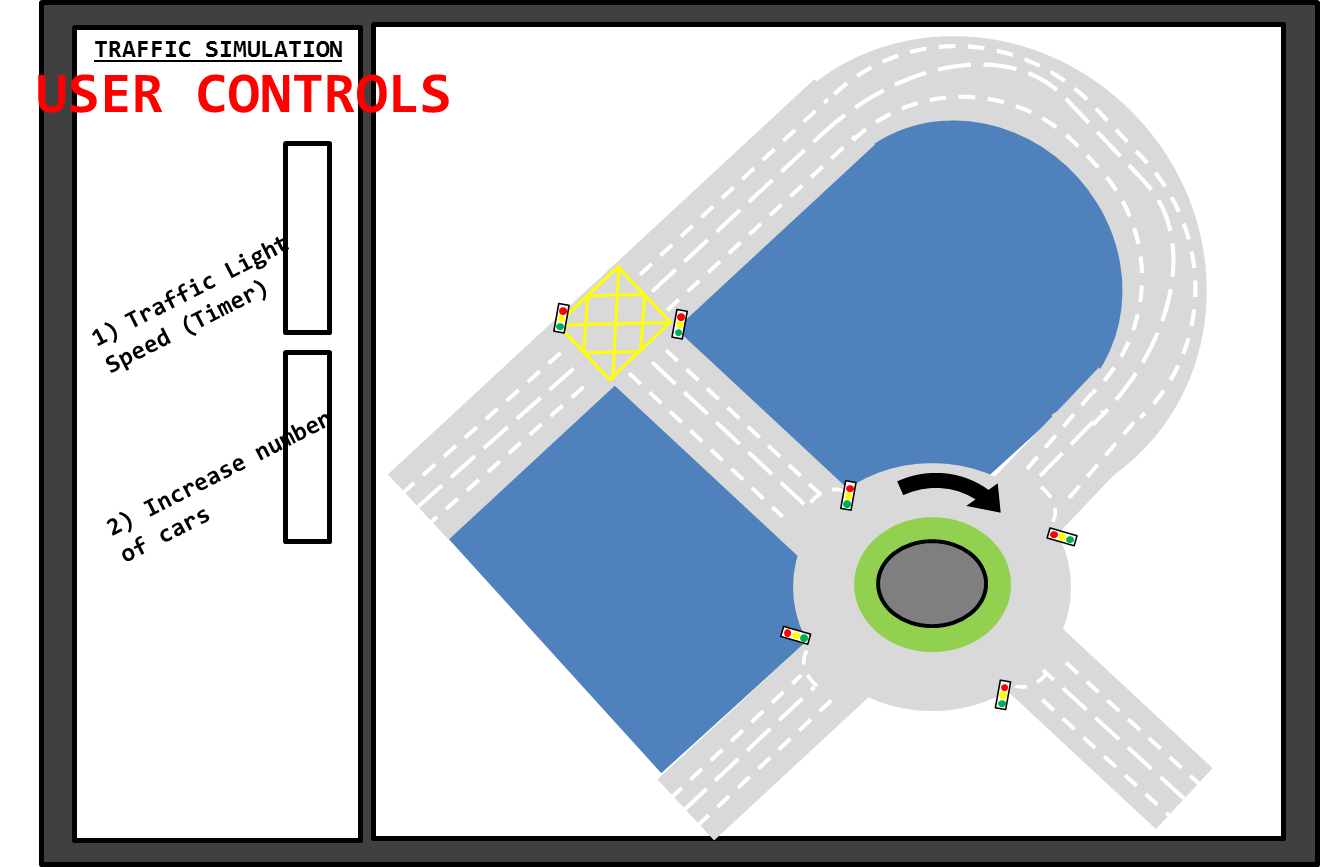
\includegraphics[width=6cm,height=4cm]{UserControls.png} 
	\captionof{figure}{GUI Design Development}
	\caption*{ }
	\label{fig:GUI}
\end{minipage}
\begin{minipage}[b]{0.45\linewidth}
	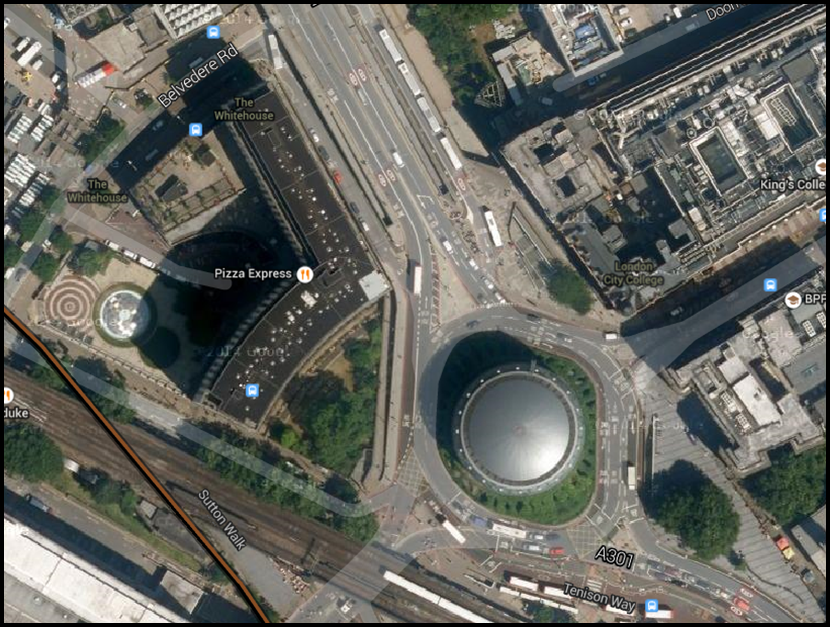
\includegraphics[width=6cm, height=4cm]{WATERLOO.png} 	\captionof{figure}{Waterloo Roundabout}
	\caption*{Source: Google Maps}
	\label{fig:Waterloo}
\end{minipage}

\end{figure}

Additionally looking at the UK Highway Code manual helped us identify the Road Marking rules and what they mean to  incorporate into our simulation. For example within our initial design Figure \ref{fig:GUI} shows rule 127 about the Centre Line "Do not cross it unless you can see the road is clear and wish to overtake or turn off" and rule 175 about Stop Lines before the traffic-lights where you must wait until the traffic-light is green.\\Overall, thus far we have created a Model-View-Controller structure for the development in Eclipse IDE and began simple road development. In terms of road development there has been doing research into the development of curved roads using analysis into B\'{e}zier Curve which are used when drawing smoothed curves between control points with anchor points on a path. B\'{e}zier Curve tracing can be solved using De Casteljau's algorithm. So in our model we will have to build an additional class 'B\'{e}zier Curve' to represent the function, essentially two polynomial functions using three points. This should help us create curved roads and enable cars to move on them to create a roundabout.\\Currently, according to the plan in Table \ref{table:plan} we are on schedule because we used the Agile development cycle, highlighting road development as the major risk making it easier to handle.

\textbf{Current Development Goals:}
\begin{enumerate}
	\item A car is able to travel on one straight road with one lane.
	\item A car is able to travel on one straight road with multiple lanes.
	\item A car should be able to travel on two roads connected with one lane in each road.
	\item A car is able to travel on two connected roads while each road can have different numbers of lanes.
\end{enumerate}

\begin{table}[ht]
	\caption{Project Plan}
	\begin{adjustwidth}{-2cm}{}
	 \footnotesize
		
		\begin{tabular}{|m{0.8cm}|m{6cm}|m{2.3cm}|m{1.3cm}|m{1.3cm}|c|m{2.6cm}|m{0.5cm}|}\hline
			
			\bf{WBS} & \bf{Task} & \bf{Predecessors} & \bf{Start Date} & \bf{Deadline} & \bf{Work Days} & \bf{Responsible} & \bf{(\%)} \\ \hline 
			1 & \multicolumn{7}{c|}{High Level Planning}  \\\hline 
			1.1 & Task Planning &  & 19/01/215 & 23/01/15 & 4 & all & 100 \\ \hline 
			1.2 & Clarify the basic function of project &  & 23/01/15 & 26/01/15 & 3 & all & 100 \\ \hline 
			1.3 & Create initial UML design ideas of system & 1.1 & 19/01/15 & 23/01/14 & 4 & all & 25 \\ \hline 
			1.4 & Determine the programming language & 1.1 & 23/01/15 & 26/02/15 & 4 & all & 100 \\\hline 
			1.5 & Intermediate Report & 1.1, 1.2, 1.4 & 26/01/15 & 02/02/15 & 9 & all & 0 \\\hline 
			2 & \multicolumn{7}{c|}{Design Stage}  \\\hline 
			2.1 & Discuss work development cycle  & 1.2 & 28/01/15 & 28/02/15 & 1 & all & 0 \\\hline 
			2.2 & Create final low level Class Diagram  & 1.2 & 26/01/15 & 30/01/15 & 3 & all & 0 \\\hline 
			2.3 & Create GUI designs  &  & 02/02/15 & 06/02/15 & 4 & all & 0 \\\hline 
			3 & \multicolumn{7}{c|}{Development Stage}  \\\hline 
			3.1 & IDE Setup (MVC) &  & 02/02/15 & 06/02/15 & 3 & Lead Programmer & 0 \\\hline 
			3.2 & Road Development  & 3.1 & 02/02/15 & 27/02/15 & 25 &  & 0 \\\hline 
			3.2.1 & Road Mathematics  &  & 02/02/15 & 13/02/15 & 11 &  & 0 \\\hline 
			3.2.2 & Road/Lane Model & 3.2.1 & 02/02/15 & 13/02/15 & 11 &  & 0 \\\hline 
			3.2.4 & Junction Development  & 3.2.1 & 02/02/15 & 27/03/15 & 25 &  & 0 \\\hline 
			3.3 & Traffic Light Development & 3.2 & 02/02/15 & 27/03/15 & 25 &  & 0 \\\hline 
			3.4 & Car Development & 3.2 & 16/02/15 & 27/03/15 & 11 &  & 0 \\\hline 
			3.5 & Testing (PHASE 1) & 3.2, 3.3, 3.4 & 27/02/15 & 06/03/15 & 7 & Testing Group & 0 \\\hline 
			3.5.2 & Quality Assurance  & 1.2, 3.2, 3.3, 3.5 & 02/02/15 & 06/03/15 & 4 &  & 0 \\\hline 
			3.6 & View (GUI) Development &  & 09/02/15 & 09/03/15 & 28 &  & 0 \\\hline 
			3.7 & Controller (GUI) Development  &  & 16/02/15 & 09/03/15 & 21 &  & 0 \\\hline 
			3.7.1 & User Change Traffic Light Speed  &  & 16/02/15 & 09/03/15 & 21 &  & 0 \\\hline 
			3.7.2 & User Change No. Of Cars.  &  & 16/02/15 & 09/03/15 & 21 &  & 0 \\\hline 
			3.8 & Testing (PHASE 2)  & 3.2, 3.5, 3.6, 3.7 & 09/03/15 & 16/03/15 & 7 & Testing Group & 0 \\\hline 
			3.8.1 & Evaluation of Final System  & 3.8 & 13/03/15 & 16/03/15 & 3 &  & 0 \\\hline 
			3.9 & Development of Additional Features & 3.8.1 & 16/03/15 & 20/03/15 & 4 &  & 0 \\\hline 
			3.10 & Final Report & 3.8.1 & 02/03/15 & 23/03/15 & 21 & all & 0 \\\hline 
			3.11 & Presentation & 3.10 & 23/03/15 & 23/03/15 & 1 & all & 0 \\ \hline 
		\end{tabular}
	\label{table:plan}
	\end{adjustwidth}
\end{table}

\section[short]{Part Two:}
\subsection{Our Team}%Tanda
We have established a number of ways to work together as a team. A key aspect we distinguished was making sure we to see each other regularly to become familiar with each other to build team relationships. This involves having two weekly meeting on Monday at 3pm and Friday at 1pm, these weekly meetings ensure that we are knowledgeable on the progress of each member in the team at the start and end of the week as well as allowing sub teams whom have been working separately to present work to all other members. Each meeting is recorded with a log that illustrates those who attended the agenda and outcome of the meeting, these minutes are recorded by the project coordinator and emailed to each member with their designated tasks for the week; additionally for casual communication a Facebook group has been set-up.

\subsubsection[short]{Roles}

\begin{itemize}%Provisional Roles
	\item Project Coordinator: Tanda Kabanda
	\item Lead Programmers: Inyeol Sohn, Jie Ding
	\item System Analysts: Qiu Yun, Mark Azer
\end{itemize}

\textbf{Note:} all group members are expected to code when designated tasks by Lead Programmers

\subsection{Collaboration}%Jie
To collaborate with others efficiently, each group member needs to focus on things they are good at. For example, someone may specialise in coding and some one at analysing, it is not a good idea to force everyone to do same work to purse the so-called 'equal'.\\The basic principle of team work is that all group members try their best on all parts they take responsibility for. Based on that, the team coordinator should assign different assignments to each member ensuring teamwork.

\subsection{Peer Assessment}%Qiu
Peer assessment is being applied in group projects,to show the individual work which based on guidelines in form of rubrics. In this group project,this assessment should based on some objects as below:

\begin{enumerate}
\item \textbf{Expression of ideas:} Showing how we going to design this traffic system including roads designing, language methods, math functions and so on, leading us to form the system from nothing to prototype. Each group member has different background, knowledge and most significantly way of thinking which is the core of group work therefore communication of ideas toward the project is worth grading.  
\item \textbf{Organization:} As a team we have a leader as organizer, who separates the jobs based on each members individual ability and creates a timetable as well as coordinate each part of the group work.
\item \textbf{Subjects:} In this specific case, means the programming and designing ,algorithms as well as organization.This part should establish how the final work formed and each ones contribution.

\end{enumerate}


\subsection{Resolving Conflicts}%Mark
During group projects conflicts are certain to happen based on the fact that we are all different. It is also important to understand that conflicts can be positive when it encourages group members to listen to each others for a new ideas which may be better for the general interest of a project. If needed group members should approach the group coordinator who must maintain a good relationship with all members to help resolve any group issues and then come to a reasonably negotiation between both parties. \\It is important that every member is respected and conflicts especially petty conflict's do not take priority. 

\end{document}
